% Created by tikzDevice version 0.12.3.1 on 2022-09-01 16:01:59
% !TEX encoding = UTF-8 Unicode
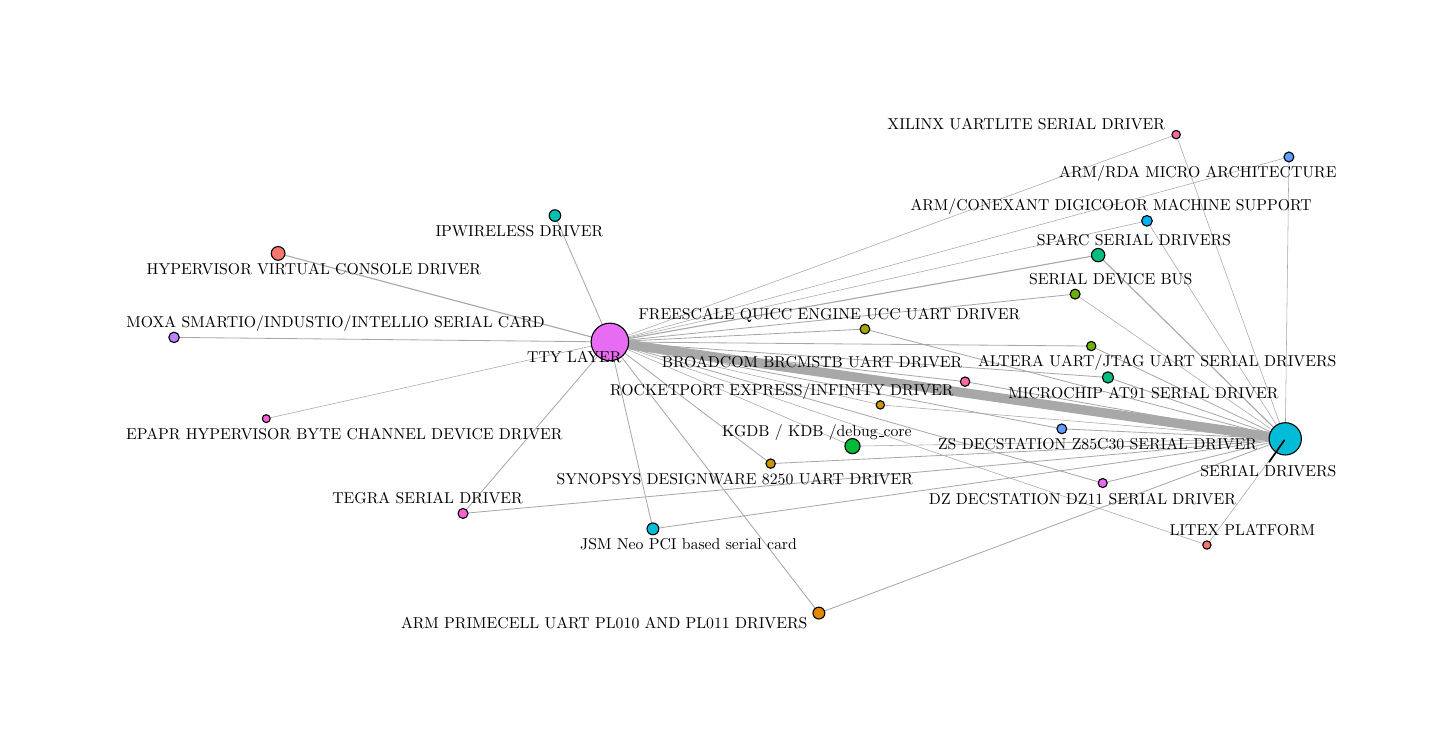
\begin{tikzpicture}[x=1pt,y=1pt]
\definecolor{fillColor}{RGB}{255,255,255}
\path[use as bounding box,fill=fillColor,fill opacity=0.00] (0,0) rectangle (505.89,252.94);
\begin{scope}
\path[clip] (  0.00,  0.00) rectangle (505.89,252.94);
\definecolor{fillColor}{RGB}{255,255,255}

\path[fill=fillColor] (  0.00,  0.00) rectangle (505.89,252.94);
\end{scope}
\begin{scope}
\path[clip] ( 32.75, 32.75) rectangle (475.89,222.94);
\definecolor{drawColor}{gray}{0.66}

\path[draw=drawColor,line width= 0.3pt,line join=round] (384.32,137.89) -- (454.42,104.36);

\path[draw=drawColor,line width= 0.3pt,line join=round] (384.32,137.89) -- (210.38,139.39);

\path[draw=drawColor,line width= 0.3pt,line join=round] (285.90, 41.40) -- (454.42,104.36);

\path[draw=drawColor,line width= 0.3pt,line join=round] (285.90, 41.40) -- (210.38,139.39);

\path[draw=drawColor,line width= 0.2pt,line join=round] (404.45,183.13) -- (454.42,104.36);

\path[draw=drawColor,line width= 0.2pt,line join=round] (404.45,183.13) -- (210.38,139.39);

\path[draw=drawColor,line width= 0.2pt,line join=round] (455.75,206.22) -- (454.42,104.36);

\path[draw=drawColor,line width= 0.2pt,line join=round] (455.75,206.22) -- (210.38,139.39);

\path[draw=drawColor,line width= 0.3pt,line join=round] (338.73,125.03) -- (454.42,104.36);

\path[draw=drawColor,line width= 0.3pt,line join=round] (338.73,125.03) -- (210.38,139.39);

\path[draw=drawColor,line width= 0.3pt,line join=round] (388.47, 88.39) -- (454.42,104.36);

\path[draw=drawColor,line width= 0.3pt,line join=round] (388.47, 88.39) -- (210.38,139.39);

\path[draw=drawColor,line width= 0.2pt,line join=round] ( 86.21,111.66) -- (210.38,139.39);

\path[draw=drawColor,line width= 0.3pt,line join=round] (302.54,144.02) -- (454.42,104.36);

\path[draw=drawColor,line width= 0.3pt,line join=round] (302.54,144.02) -- (210.38,139.39);

\path[draw=drawColor,line width= 0.4pt,line join=round] ( 90.50,171.37) -- (210.38,139.39);

\path[draw=drawColor,line width= 0.3pt,line join=round] (190.52,185.05) -- (210.38,139.39);

\path[draw=drawColor,line width= 0.3pt,line join=round] (225.92, 71.83) -- (454.42,104.36);

\path[draw=drawColor,line width= 0.3pt,line join=round] (225.92, 71.83) -- (210.38,139.39);

\path[draw=drawColor,line width= 0.2pt,line join=round] (298.04,101.72) -- (454.42,104.36);

\path[draw=drawColor,line width= 0.2pt,line join=round] (298.04,101.72) -- (210.38,139.39);

\path[draw=drawColor,line width= 0.2pt,line join=round] (426.11, 66.00) -- (454.42,104.36);

\path[draw=drawColor,line width= 0.2pt,line join=round] (426.11, 66.00) -- (210.38,139.39);

\path[draw=drawColor,line width= 0.3pt,line join=round] (390.36,126.55) -- (454.42,104.36);

\path[draw=drawColor,line width= 0.3pt,line join=round] (390.36,126.55) -- (210.38,139.39);

\path[draw=drawColor,line width= 0.3pt,line join=round] ( 52.89,141.02) -- (210.38,139.39);

\path[draw=drawColor,line width= 0.2pt,line join=round] (308.10,116.63) -- (454.42,104.36);

\path[draw=drawColor,line width= 0.2pt,line join=round] (308.10,116.63) -- (210.38,139.39);

\path[draw=drawColor,line width= 0.2pt,line join=round] (378.49,156.66) -- (454.42,104.36);

\path[draw=drawColor,line width= 0.3pt,line join=round] (378.49,156.66) -- (210.38,139.39);

\path[draw=drawColor,line width= 0.4pt,line join=round] (454.42,104.36) -- (386.81,170.75);

\path[draw=drawColor,line width= 0.3pt,line join=round] (454.42,104.36) -- (268.47, 95.41);

\path[draw=drawColor,line width= 0.3pt,line join=round] (454.42,104.36) -- (157.31, 77.41);

\path[draw=drawColor,line width= 3.4pt,line join=round] (454.42,104.36) -- (210.38,139.39);

\path[draw=drawColor,line width= 0.2pt,line join=round] (454.42,104.36) -- (415.00,214.30);

\path[draw=drawColor,line width= 0.3pt,line join=round] (454.42,104.36) -- (373.68,107.97);

\path[draw=drawColor,line width= 0.4pt,line join=round] (386.81,170.75) -- (210.38,139.39);

\path[draw=drawColor,line width= 0.3pt,line join=round] (268.47, 95.41) -- (210.38,139.39);

\path[draw=drawColor,line width= 0.3pt,line join=round] (157.31, 77.41) -- (210.38,139.39);

\path[draw=drawColor,line width= 0.2pt,line join=round] (210.38,139.39) -- (415.00,214.30);

\path[draw=drawColor,line width= 0.3pt,line join=round] (210.38,139.39) -- (373.68,107.97);
\definecolor{drawColor}{RGB}{0,0,0}
\definecolor{fillColor}{RGB}{107,177,0}

\path[draw=drawColor,line width= 0.4pt,line join=round,line cap=round,fill=fillColor] (384.32,137.89) circle (  1.68);
\definecolor{fillColor}{RGB}{229,135,0}

\path[draw=drawColor,line width= 0.4pt,line join=round,line cap=round,fill=fillColor] (285.90, 41.40) circle (  2.14);
\definecolor{fillColor}{RGB}{0,176,246}

\path[draw=drawColor,line width= 0.4pt,line join=round,line cap=round,fill=fillColor] (404.45,183.13) circle (  1.93);
\definecolor{fillColor}{RGB}{97,156,255}

\path[draw=drawColor,line width= 0.4pt,line join=round,line cap=round,fill=fillColor] (455.75,206.22) circle (  1.79);
\definecolor{fillColor}{RGB}{255,103,164}

\path[draw=drawColor,line width= 0.4pt,line join=round,line cap=round,fill=fillColor] (338.73,125.03) circle (  1.70);
\definecolor{fillColor}{RGB}{231,107,243}

\path[draw=drawColor,line width= 0.4pt,line join=round,line cap=round,fill=fillColor] (388.47, 88.39) circle (  1.63);
\definecolor{fillColor}{RGB}{253,97,209}

\path[draw=drawColor,line width= 0.4pt,line join=round,line cap=round,fill=fillColor] ( 86.21,111.66) circle (  1.43);
\definecolor{fillColor}{RGB}{163,165,0}

\path[draw=drawColor,line width= 0.4pt,line join=round,line cap=round,fill=fillColor] (302.54,144.02) circle (  1.76);
\definecolor{fillColor}{RGB}{248,118,109}

\path[draw=drawColor,line width= 0.4pt,line join=round,line cap=round,fill=fillColor] ( 90.50,171.37) circle (  2.48);
\definecolor{fillColor}{RGB}{0,192,175}

\path[draw=drawColor,line width= 0.4pt,line join=round,line cap=round,fill=fillColor] (190.52,185.05) circle (  2.09);
\definecolor{fillColor}{RGB}{0,188,216}

\path[draw=drawColor,line width= 0.4pt,line join=round,line cap=round,fill=fillColor] (225.92, 71.83) circle (  2.13);
\definecolor{fillColor}{RGB}{0,186,56}

\path[draw=drawColor,line width= 0.4pt,line join=round,line cap=round,fill=fillColor] (298.04,101.72) circle (  2.73);
\definecolor{fillColor}{RGB}{248,118,109}

\path[draw=drawColor,line width= 0.4pt,line join=round,line cap=round,fill=fillColor] (426.11, 66.00) circle (  1.50);
\definecolor{fillColor}{RGB}{0,191,125}

\path[draw=drawColor,line width= 0.4pt,line join=round,line cap=round,fill=fillColor] (390.36,126.55) circle (  2.04);
\definecolor{fillColor}{RGB}{185,131,255}

\path[draw=drawColor,line width= 0.4pt,line join=round,line cap=round,fill=fillColor] ( 52.89,141.02) circle (  1.89);
\definecolor{fillColor}{RGB}{201,152,0}

\path[draw=drawColor,line width= 0.4pt,line join=round,line cap=round,fill=fillColor] (308.10,116.63) circle (  1.51);
\definecolor{fillColor}{RGB}{107,177,0}

\path[draw=drawColor,line width= 0.4pt,line join=round,line cap=round,fill=fillColor] (378.49,156.66) circle (  1.80);
\definecolor{fillColor}{RGB}{0,188,216}

\path[draw=drawColor,line width= 0.4pt,line join=round,line cap=round,fill=fillColor] (454.42,104.36) circle (  5.83);
\definecolor{fillColor}{RGB}{0,191,125}

\path[draw=drawColor,line width= 0.4pt,line join=round,line cap=round,fill=fillColor] (386.81,170.75) circle (  2.41);
\definecolor{fillColor}{RGB}{201,152,0}

\path[draw=drawColor,line width= 0.4pt,line join=round,line cap=round,fill=fillColor] (268.47, 95.41) circle (  1.70);
\definecolor{fillColor}{RGB}{253,97,209}

\path[draw=drawColor,line width= 0.4pt,line join=round,line cap=round,fill=fillColor] (157.31, 77.41) circle (  1.80);
\definecolor{fillColor}{RGB}{231,107,243}

\path[draw=drawColor,line width= 0.4pt,line join=round,line cap=round,fill=fillColor] (210.38,139.39) circle (  6.78);
\definecolor{fillColor}{RGB}{255,103,164}

\path[draw=drawColor,line width= 0.4pt,line join=round,line cap=round,fill=fillColor] (415.00,214.30) circle (  1.52);
\definecolor{fillColor}{RGB}{97,156,255}

\path[draw=drawColor,line width= 0.4pt,line join=round,line cap=round,fill=fillColor] (373.68,107.97) circle (  1.77);

\path[draw=drawColor,line width= 0.6pt,line join=round,line cap=round] (448.62, 96.00) -- (454.06,103.84);

\node[text=drawColor,anchor=base,inner sep=0pt, outer sep=0pt, scale=  0.57] at (408.17,130.43) {ALTERA UART/JTAG UART SERIAL DRIVERS};

\node[text=drawColor,anchor=base,inner sep=0pt, outer sep=0pt, scale=  0.57] at (208.34, 35.76) {ARM PRIMECELL UART PL010 AND PL011 DRIVERS};

\node[text=drawColor,anchor=base,inner sep=0pt, outer sep=0pt, scale=  0.57] at (391.52,186.70) {ARM/CONEXANT DIGICOLOR MACHINE SUPPORT};

\node[text=drawColor,anchor=base,inner sep=0pt, outer sep=0pt, scale=  0.57] at (422.86,198.76) {ARM/RDA MICRO ARCHITECTURE};

\node[text=drawColor,anchor=base,inner sep=0pt, outer sep=0pt, scale=  0.57] at (283.44,130.15) {BROADCOM BRCMSTB UART DRIVER};

\node[text=drawColor,anchor=base,inner sep=0pt, outer sep=0pt, scale=  0.57] at (381.14, 80.59) {DZ DECSTATION DZ11 SERIAL DRIVER};

\node[text=drawColor,anchor=base,inner sep=0pt, outer sep=0pt, scale=  0.57] at (114.43,104.19) {EPAPR HYPERVISOR BYTE CHANNEL DEVICE DRIVER};

\node[text=drawColor,anchor=base,inner sep=0pt, outer sep=0pt, scale=  0.57] at (289.69,147.59) {FREESCALE QUICC ENGINE UCC UART DRIVER};

\node[text=drawColor,anchor=base,inner sep=0pt, outer sep=0pt, scale=  0.57] at (103.42,163.86) {HYPERVISOR VIRTUAL CONSOLE DRIVER};

\node[text=drawColor,anchor=base,inner sep=0pt, outer sep=0pt, scale=  0.57] at (177.66,177.58) {IPWIRELESS DRIVER};

\node[text=drawColor,anchor=base,inner sep=0pt, outer sep=0pt, scale=  0.57] at (238.81, 64.33) {JSM Neo PCI based serial card};

\node[text=drawColor,anchor=base,inner sep=0pt, outer sep=0pt, scale=  0.57] at (285.19,105.29) {KGDB / KDB /debug{\_{}}core};

\node[text=drawColor,anchor=base,inner sep=0pt, outer sep=0pt, scale=  0.57] at (438.93, 69.56) {LITEX PLATFORM};

\node[text=drawColor,anchor=base,inner sep=0pt, outer sep=0pt, scale=  0.57] at (403.18,119.07) {MICROCHIP AT91 SERIAL DRIVER};

\node[text=drawColor,anchor=base,inner sep=0pt, outer sep=0pt, scale=  0.57] at (111.25,144.56) {MOXA SMARTIO/INDUSTIO/INTELLIO SERIAL CARD};

\node[text=drawColor,anchor=base,inner sep=0pt, outer sep=0pt, scale=  0.57] at (272.54,120.20) {ROCKETPORT EXPRESS/INFINITY DRIVER};

\node[text=drawColor,anchor=base,inner sep=0pt, outer sep=0pt, scale=  0.57] at (391.35,160.23) {SERIAL DEVICE BUS};

\node[text=drawColor,anchor=base,inner sep=0pt, outer sep=0pt, scale=  0.57] at (448.34, 90.58) {SERIAL DRIVERS};

\node[text=drawColor,anchor=base,inner sep=0pt, outer sep=0pt, scale=  0.57] at (399.75,174.35) {SPARC SERIAL DRIVERS};

\node[text=drawColor,anchor=base,inner sep=0pt, outer sep=0pt, scale=  0.57] at (255.50, 87.89) {SYNOPSYS DESIGNWARE 8250 UART DRIVER};

\node[text=drawColor,anchor=base,inner sep=0pt, outer sep=0pt, scale=  0.57] at (144.51, 80.96) {TEGRA SERIAL DRIVER};

\node[text=drawColor,anchor=base,inner sep=0pt, outer sep=0pt, scale=  0.57] at (197.55,131.91) {TTY LAYER};

\node[text=drawColor,anchor=base,inner sep=0pt, outer sep=0pt, scale=  0.57] at (360.85,216.00) {XILINX UARTLITE SERIAL DRIVER};

\node[text=drawColor,anchor=base,inner sep=0pt, outer sep=0pt, scale=  0.57] at (386.58,100.49) {ZS DECSTATION Z85C30 SERIAL DRIVER};
\end{scope}
\end{tikzpicture}
